\chapter{Prezentacja aplikacji}
W niniejszym rozdziale zostanie zaprezentowany od strony użytkowej system, który powstał w ramach niniejszej pracy.

W momencie rozpoczęcia nowej sesji, użytkownikowi pokazuje się ekran logowania:

\begin{figure} [H]
    \begin{center}
	
\includegraphics[scale=.6]{img/ekranLogowania.png}
	\caption{Ekran logowania}
	\label{stronaPrzyklad}
    \end{center}
\end{figure}

Następnie, bo zalogowaniu, użytkownikowi jest wyświetlane okno wyboru opracowania (na poniższym rysunku). Ekran ten jest widoczny na samym początku sesji, ale może też być wyświetlony w dowolnym momencie użytkowania systemu, poprzez kliknięcie przycisku "Zmień" w sekcji opracowanie, w górnej belce strony. Z poziomu wyświetlonego ekranu użytkownik może dodawać, edytować bądź usuwać (tylko te, dla których nie zostały dodane żadne dane) opracowania. W ten sposób jest spełniony przypadek użycia UC1. - Zarządzaj listą opracowań.
\begin{figure} [H]
    \begin{center}
	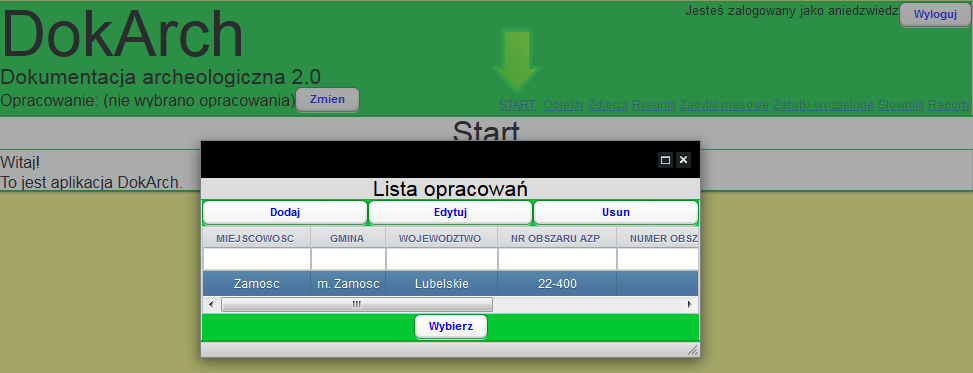
\includegraphics[scale=.6]{img/ekranStartowy.png}
	\caption{Ekran logowania}
	\label{stronaPrzyklad}
    \end{center}
\end{figure}
\newpage
Standardowy ekran aplikacji wyświetlający liste elementów wygląda jak na poniższym rysunku.

\begin{figure} [H]
    \begin{center}
	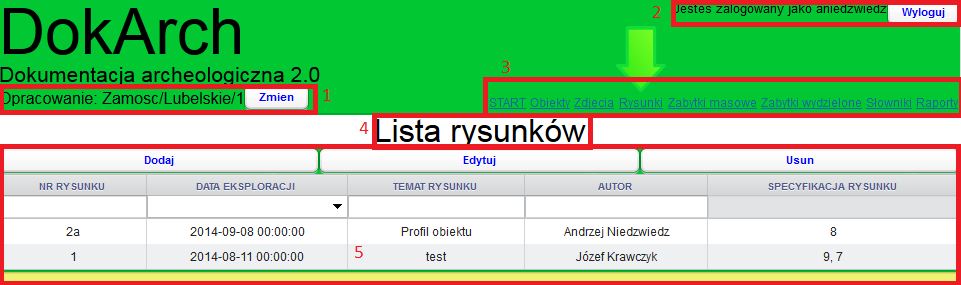
\includegraphics[scale=.6]{img/strona.png}
	\caption{Przykładowa podstrona systemu}
	\label{stronaPrzyklad}
    \end{center}
\end{figure}

Na załączonym obrazku widać, że strona aplikacji składa się z:
\begin{itemize}
\item górnej belki zawierającej w sobie informacje o bieżącym opracowaniu (1 na rysunku), informacje o zalogowanym użytkowniku (2) oraz menu (3)
\item belki tytułowej (4)
\item głównej treści strony (5) 
\end{itemize}

Powyższy rysunek demonstruje także przykładowy widok listujący wprowadzone dane (w tym przypadku rysunki). Dzięki addonowi FilterTable, możliwe jest filtrowanie widocznych elementów po ich zawartości w konkretnych polach. Standardowa funkcjonalność Vaadina pozwala także sortować wiersze wg wartości w kolumnie - w tym celu wystarczy kliknąć nagłówek kolumny.

\begin{figure} [H]
    \begin{center}
	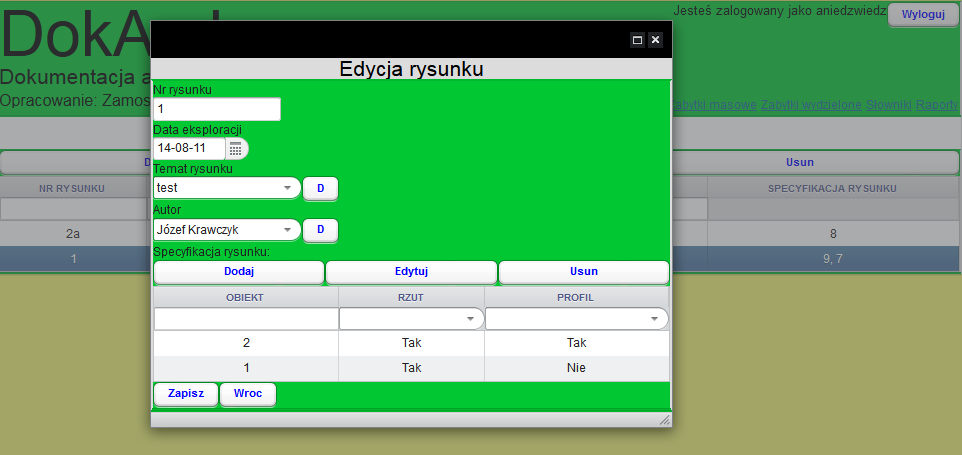
\includegraphics[scale=.6]{img/edycja.png}
	\caption{Przykładowa edycja obiektu dokumentacyjnego}
	\label{edycjaPrzyklad}
    \end{center}
\end{figure}

\newpage
Rysunek znajdujący się nad tym tekstem demonstruje ekran edycji wiersza (w tym przypadku wiersz odzwierciedla ewidencjonowany rysunek). Ten sam ekran (tylko z niewypelnionymi wartościami) jest wyświetlany użytkownikowi po otrzymaniu informacji o wciśnięciu przez użytkownika przycisku dodaj. Lista wysunków wraz z oknem edycji rysunków wypełniają przypadek użycia "UC5. Zarządzaj rysunkami".

\begin{figure} [H]
    \begin{center}
	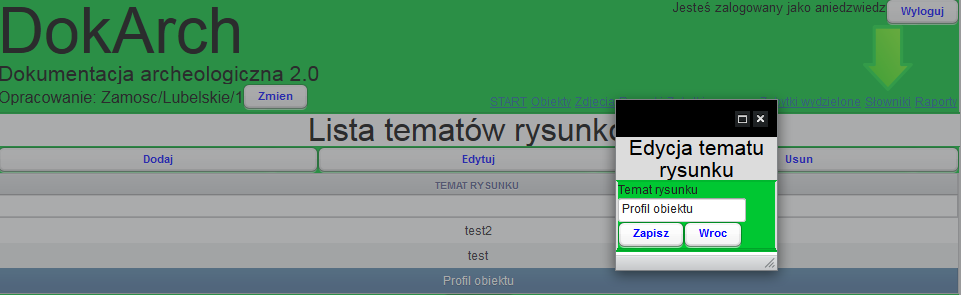
\includegraphics[scale=.6]{img/edycjaSlownika.png}
	\caption{Przykładowa edycja słownika}
	\label{edycjaSlownika}
    \end{center}
\end{figure}

Rysunek powyżej przedstawia standardowy sposób edycji słownika (wybranie w menu w górnej belce "Słowniki" a następnie wybranie słownika "Tematy rysunków"). Jest to jeden ze sposobów modyfikacji wartości słownika.

\begin{figure} [H]
    \begin{center}
	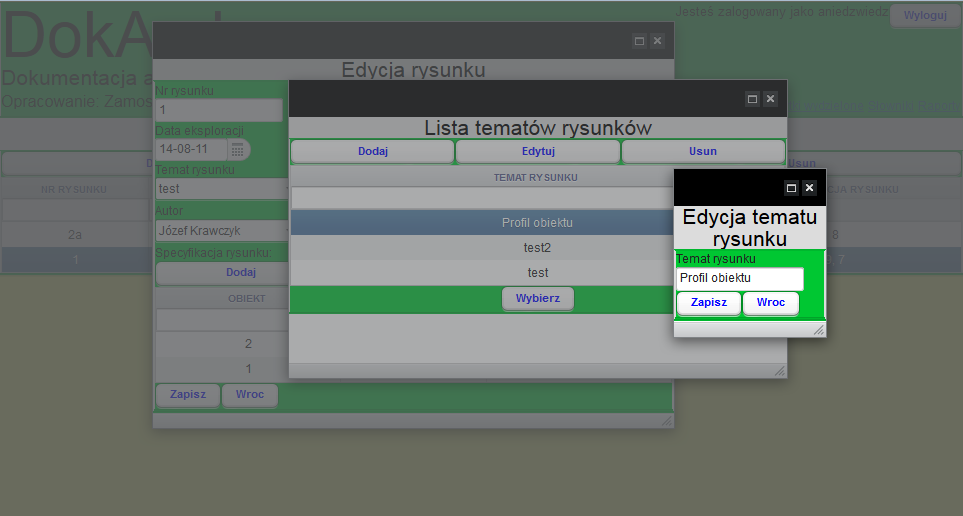
\includegraphics[scale=.6]{img/edycjaSlownikaWLocie.png}
	\caption{Przykładowa edycja słownika w trakcie edycji obiektu go używającego}
	\label{edycjaSlownikaWLocie}
    \end{center}
\end{figure}

\newpage
Powyżej został przedstawiony ekran modyfikacji słownika w ``locie", czyli w trakcie edycji wiersza, który zawiera wartość ze słownika. Możliwe jest dynamiczne wprowadzanie wartości bez konieczności zamykania okna edycji.

Wyświetlenie listy wartości oraz ich modyfikacja może nastąpić na dwa sposoby. Pierwszy sposób to wybranie przycisku D przy polu słownikowym. Wtedy otwiera się okno z tabelką widoczne poniżej:

\begin{figure} [H]
    \begin{center}
	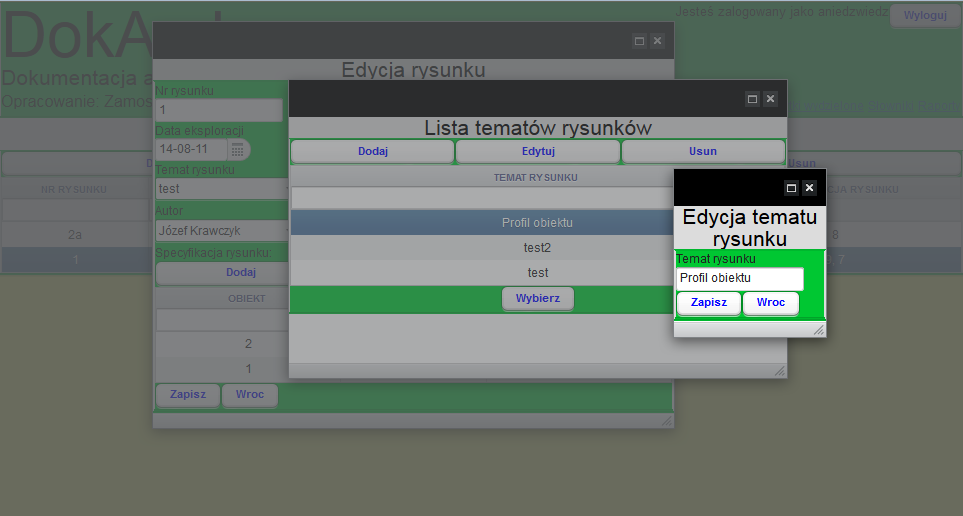
\includegraphics[scale=.6]{img/edycjaSlownikaWLocie.png}
	\caption{Lista tematów rysunków zmieniana w ``locie''}
	\label{edycjaListySlownikaWLocie}
    \end{center}
\end{figure}

Drugim sposobem jest kliknięcie w link w menu strony w nazwie "Słowniki". Link ten przeniesie użytkownika do strony widocznej poniżej:

\begin{figure} [H]
    \begin{center}
	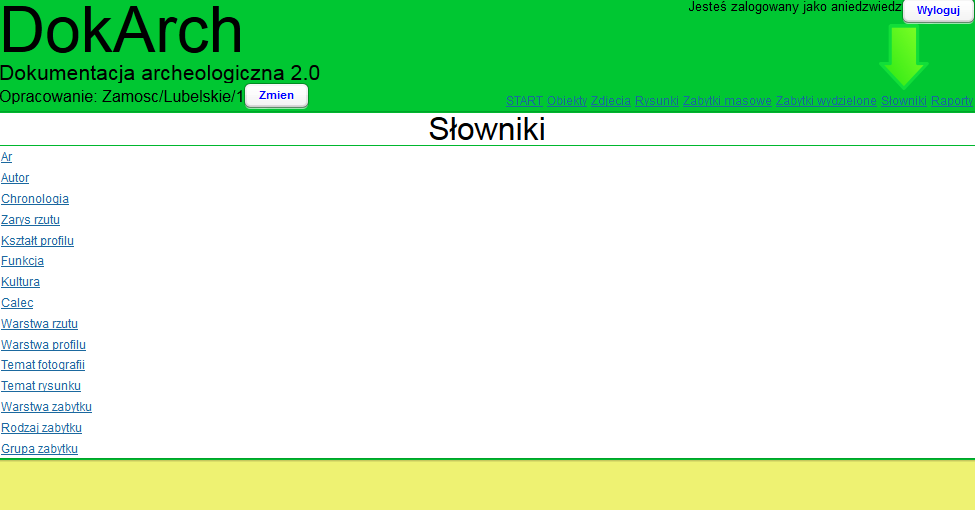
\includegraphics[scale=.6]{img/listaSlownikow.png}
	\caption{Lista słowników}
	\label{listaSlownikow}
    \end{center}
\end{figure}
\newpage
Następnie użytkownik wybiera interesujący go słownik i klika w link prowadzący do niego. Przykładowy słownik po wciśnięciu linka:

\begin{figure} [H]
    \begin{center}
	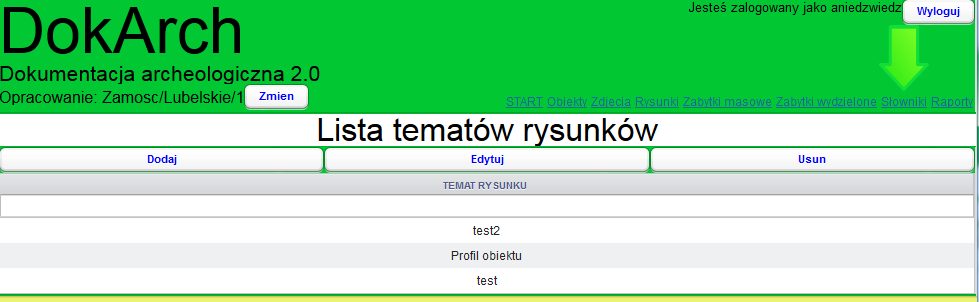
\includegraphics[scale=.6]{img/listaTematowRysunkow.png}
	\caption{Lista tematów rysunków}
	\label{listaTematowRysunkow}
    \end{center}
\end{figure}

W ten sposób pokazano, że system ma zaimplementowany przypadek użycia UC9. Zarządzaj tematami rysunków.

System potrafi także generować raporty. Aby tego dokonać wystarczy kliknąc link w menu "Raporty", i wybrać interesujący raport z listy:

\begin{figure} [H]
    \begin{center}
	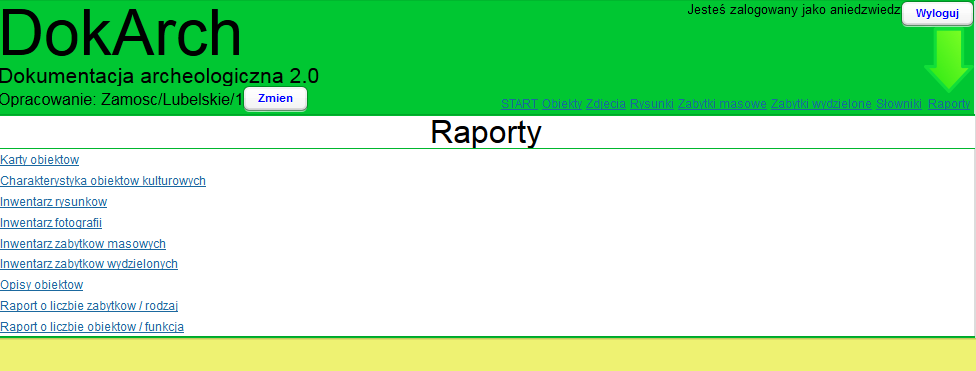
\includegraphics[scale=.6]{img/ekranRaportow.png}
	\caption{Ekran raportów}
	\label{listaRaportow}
    \end{center}
\end{figure}
\newpage
Przykładowy raport wygenerowany przez system:

\begin{figure} [H]
    \begin{center}
	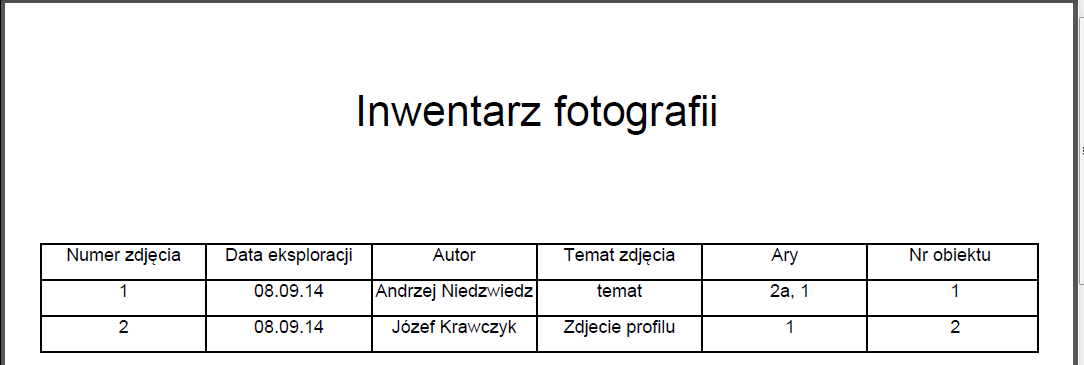
\includegraphics[scale=.6]{img/przykladowyRaport.png}
	\caption{Przykładowy raport}
	\label{przykladowyRaport}
    \end{center}
\end{figure}

% ex: set tabstop=4 shiftwidth=4 softtabstop=4 noexpandtab fileformat=unix filetype=tex spelllang=pl,en spell: